\chapter{Simulation}

\section{Parameters}

All parameters of the simulation have been regrouped into a single configuration \texttt{JSON} file with a hierarchy based on the models (each one will read the values it needs). Whenever we are testing one configuration of the simulation, we can simply modify the values of this file to see the consequences of such modifications compared to the template version (\texttt{params/templateExperiments.json}). The default file looks like as shown in the following figure and all parameters will be explained in the following sections.

\begin{lstlisting}[language=json,firstnumber=1]
{
    "World": {
        "PRODUCT_CHOICE": "CHEAPEST",
        "NB_STATES": 200,
        "NB_AGENTS": 30000,
        "NB_TICKS": 4000,
        "NB_TICKS_SAVE_CSV": 100
    },
    "Connections": {
        "CLUSTER_SIZE": 0,
        "PROB_CONNECTION": 0.0
    },
    "State": {
        "Tax": {
            "MIN_VAT": 0.2,
            "MAX_VAT": 0.2,
            "MIN_LEVY": 0.1,
            "MAX_LEVY": 0.1,
            "MIN_TARIFF": 0.3,
            "MAX_TARIFF": 0.3,
            "VAL_WEALTH_TAX_TOP": 0.1,
            "MIN_WEALTH_TAX_VALUE": 0.2,
            "MAX_WEALTH_TAX_VALUE": 0.2,
            "NB_TICKS_COLLECT_TAXES": 100
        },
        "Allowance": {
            "NB_TICKS_DISTRIBUTE_ALLOWANCES": 100
        },
        "Others": {
            "MIN_UNEMPLOYMENT": 0.05,
            "MAX_UNEMPLOYMENT": 0.05,
            "MIN_BLACK": 0.15,
            "MAX_BLACK": 0.15
        }
    },
    "Agent": {
        "MIN_INIT_MONEY": 1000.0,
        "MAX_INIT_MONEY": 1000.0,
        "RATIO_BUY": 0.5,
        "RATIO_PRODUCE": 0.5
    },
    "Product": {
        "NB_DIFF_PRODUCTS": 50,
        "MIN_PRICE": 0.0,
        "MAX_PRICE": 300.0,
        "MAX_STOCK": 2000
    }
}
\end{lstlisting}

\section{Main}

    The simulation has been coded using Java 16 for its large range of libraries, robustness, rapidness (compared to Python for instance), its strongly typed paradigm and, of course, because of its Object Oriented Programming paradigm (OOP) which fits how we will code our models (see next section). 

    Everything starts with the \texttt{Main.java} file. Multiple simulations can be ran in parallel thanks to the use of threads (one simulation = one World = one thread). Each line in the \texttt{params/configs.txt} file corresponds to one configuration (thus one \texttt{.json} file containing all the parameters located in the \texttt{params} directory) that will be launch. For instance:

    \begin{lstlisting}[language=json,firstnumber=1]
experiment1.json
experiment2.json
experiment3.json
    \end{lstlisting}



\section{Models}\label{section:models}

ABM provides numerous benefits, as stated before. Amongst these, we can cite two key points that motivate this thesis: \textquote{ABM captures emergent phenomena and it provides a natural description of a system}. This is important because our goal is to have an empirical understanding of our system \cite{tesfatsion_handbook}, i.e., we want to understand why some systems work while others do not. And this will be done with in very intuitive way based on a natural description of ours models which will interact.

Nonetheless, we should also note some drawbacks of this approach; especially the issues revolving around social sciences such as irrational behavior or subjective choices which are difficult to quantify and pin down mathematically \cite{ABM}. In order to simulate some irrational behavior, we could introduce some non-deterministic behavior where the agents would make a random choice from time to time. However, such a stochastic behavior will be hard to calibrate. 
Another problem that may rise is the required computational power. Simulating such a complex system made of different models with many thousands agents is expensive. Therefore, we shall use tools that allow us to perform heavy computations as described in the implementation section~\ref{section:implementation}. 

We will now focus on the different models that make up our economical system: the World, the WorldMarket, the States, the Market, the Agents and the Products. We will start by the smallest entity until the biggest: from Products to the World.


\subsection{Product}\label{section:product}
In the real world, we have two different types of products: the goods and the services. However, in this paper, we will not distinguish these two terms because the only thing that matters is that one producer and one consumer perform an exchange of a product in return of a certain amount of money. From now on, we will use the word \emph{product} to encompass these two words.

Each Product belongs to one Agent has a type (which is a simple number) to represent different kinds of products (apples, clothes, cars, ...), a default selling price (which will be updated by the Agent according to its skills) and the stock units.

We should also note that by "exchange of product", we mean a sale-purchase relationship: after receiving the money, the producer does not have any right on the sold product anymore as opposed to a location or a license. We also assume that any product sold is directly consumed by the buyer.

\subsection{Agent}\label{section:agent}
We will focus on four key aspects of an agent: its assets, its actions and its skills. Each agent is unique. This will allow us to have an heterogeneous 'society' similarly to the one in which we live where each and every one of us has some assets and different skills.

    \subsubsection{Assets}\label{section:assets}
    Usually an agent owns multiple and different types of assets. In our case, we will focus on the financial and material ones. Indeed, an agent has a certain amount of money on its bank account. This amount is, needless to say, variable. 
    However, each agent will start the simulation with a certain amount of money and afterwards, it will be up to it to spend it as it wishes and also increase it by selling the products it produces (see section about skills~\ref{section:skills}). 
    The amount of money an agent has will play a key part in the statistics that we will compute in order to study our study (for example to study the wealth distribution amongst agents). 

    Our agent will also have material assets, namely the products it produces. It can only produce one type of products as described in section about skills~\ref{section:skills}. By producing a unit of a certain type of product, we increase the stock the agent has of that product. And, similarly, by selling a unit of a product, we decrease the stock if it was not empty. We can note that there is a lower bound (0 unit), and an upper bound depending on the parameter \texttt{Product.MAX\_STOCK}.


    \subsubsection{Actions}\label{section:actions}
    An agent can be seen as a person who has both duties and rights. The agent \emph{can} produce, make a transaction (which encompasses the selling and buying actions) and consume products. These actions belong to the rights of the agent. Performing any of those actions will involve different components: a product, some money, a buyer (or consumer) and a seller (or producer) and the States to which our agents belong. 

    However, we should also note that an agent has duties. Indeed, in our system we will introduce the concept of State (in the section~\ref{section:state}). Because an agent belongs to a State, it \emph{has} to pay certain taxes. 
    For instance, the well-known VAT (Value Added Tax) which has to be payed to the State each time an agent \emph{sells} a product. The rate the VAT will be State-dependent. Depending on the State, we may have different taxes that we will study to see how they influence our system. All these taxes are examples of duties an agent has. 

    The actions involving a product are described as followed:

    \paragraph{Produce}
    Producing is the primary goal of an agent. At first, the Agent chooses one Product type to produce. Depending on its \emph{talent} (a random value between 0 and 1), the Agent will be able to reduce the default selling price of that product as: 

    $$Product.sellingPrice = (1-talent) \cdot Product.defaultSellingPrice$$

    So the more talent an agent has, the smaller the price of the product will be and therefore the more chances this product will be bought by other agents. On the other side, it has decided that there are no production price because otherwise, tick after tick, money would 'leak' out of the System until no agent is able to buy or produce which would be counterproductive for the experiments.

    However, an agent will not be able to produce at each time step (a tick as described in section~\ref{section:world}). This will allow other agents (buyers, i.e., consumers) to have some time to buy our agent's products. Indeed, our agent should not produce all the time in order to avoid having too many stocks of unsold products. An agent will not be able to produce indefinitely, we have an upper bound: the max stock allowed by the parameters (\texttt{Product.MAX\_STOCK}).

    \paragraph{Buy} 
    An agent does not buy at every time step (tick), but when it does, it will analyse all its possibilities. It will choose one product it needs and try to find a seller. For this, we will analyze all the sellers and rank their products by price. This will be detailed in the Market section.


\subsection{State}\label{section:state}
In this work, we introduce a new concept of 'State' which we will define as an entity containing multiple agents constituting a community operating on the same sets of rules.

    \subsubsection{Rights and duties}
    All of the agents in our simulation will be assigned to only one State: an many-to-one kind of relationship (multiple agents belong to one State). As stated previously, agents have some duties towards the State they belong to: taxes.

        \paragraph{Duties}
            Whenever an agent sells a product to another agent, it has to pay a certain amount to the State to which it belongs. This is an already existing concept: the Value Added Tax (VAT). This amount is computed as a percentage of the product's price. The VAT's value will be decided by the State. Other taxes have been introduced too:

            \begin{itemize}
                \item the levy which is a contribution to the State. This levy will happen every time a certain number of ticks have been performed. The amount of this levy is fixed according to a certain percentage of the financial assets of an agent.
                \item custom tariffs which will discourage buying from non-connected States as they penalize the price of a Product sold by another State with which there is no connection.
                \item a wealth tax which will not be payed by all agents, only the wealthiest. This tax is optional and not all States will impose it. It will be obligatory for the top 10\% richest agents.
            \end{itemize}

            The default values of these taxes were chosen to be close to the averages of the OECD's.

        \paragraph{Rights}
            However, they also have some rights in regards to the State that are split in two categories: allowances and a universal basic income (which is in fact a particular case of allowances). Each State may choose to use exclusively one of them.

            \subparagraph{Universal Basic Income}
                The simplest case is the universal basic income which does not make any distinction between the agents. Every agent belonging to the same State will receive the same amount of fictional money (what is called the \texttt{Flat} allowance in the code). Therefore we simply divide the money of the State by the number of agents it has and every agent receives the same share of money.
            

            \subparagraph{Allowance}
                The amount of an allowance will depend greatly on the wealthiness of its receiver because its goals is to distribute wealth (what is called the \texttt{Fair} allowance in the code). To compute the amount that each Agent receives, we have to take into account the following three conditions:
                
                \begin{itemize}
                    \item The State cannot distribute more money than it has
                    \item The wealthiest agents should still be wealthier (thus, the order of agent's wealth should stay the same, i.e. the poorest agent cannot suddenly become the richest after allowances have been distributed). 
                    \item Wealth is distributed more evenly among agents.
                \end{itemize}

                For this, I have decided to use the following methodology:

                \begin{enumerate}
                    \item Compute the average money of an agent
                    \item Compute, for each agent, the difference between its money and the average. If the Agent has more money than the average, the difference will be set to zero.
                    \item Now we know how much money the State has to distribute. However we have two cases that might happen: either the State has enough money, or not.
                    \item If the State has enough money, we simply give each Agent its computed difference with the average, and divide the rest of the money the State has equally between all agents.
                    \item If the State has not enough money, we compute the share of an agent based on a simple computation: $\frac{\text{stateMoneyToDistribute} \cdot \text{difference}}{\text{totalToDistribute}}$. This guarantees the State does not spend more money than it has, while reducing inequalities.
                \end{enumerate}

                \subparagraph{Example}
                The State has 100 units of money to distribute among 4 agents. Currently, A is the poorest and has 10 units of money, B 20, C 100 and D 170. The Gini coefficient is equal to 0.467 and the average money of an agent is therefore $\frac{10 + 20 + 100 + 170}{4} = 75$. Hence A's difference is thus $75-10=65$, B's 55, C's 0 and D's 0. However, the State does not have sufficient money to pay both A and B (total of 120, yet the State has only 100). Thus, A will receive $\frac{100 \cdot 65}{120} \approx 54.1$, and B $\frac{100 \cdot 55}{120} \approx 45.8$. The total distributed money is therefore 100, and the inequalities between agents has been reduced: A, B, C have 100, D has 170. This respects our three conditions from earlier and the Gini coefficient is equal to 0.112 (closer to 0 means more equality)


        \paragraph{Wealth distribution}
        The taxes and allowances are introduced in order to limit the money difference between the richest and poorest agents and allow a better distribution of the wealth in the system. Because all these parameters are adjustable, different type of States will emerge.

        Traditionally, States can, very roughly, be divided in three categories: pure socialism, pure capitalism or mixed. If a State decides to collect no taxes and offer absolutely no wealth distribution, we would label it as a pure capitalist economy. Conversely, if a State decides to opt for a planned economy (or pure socialism), every agent would work for the State it belongs to, and would not be able to increase its own financial assets because the taxes are too high for instance in our simulation.
        However, most real markets today are not that extreme and fall into the mixed market category where some wealth distribution is present. This is a very simplified classification but it will suffice in our case to study and understand our simulation.

        Wealth distribution will be one of the key factors when we will analyse the simulation.


    \subsubsection{Black economy}
    The black economy is a share of the economy from which the State gets no tax. This is a parameter of the System and each State has one value in between 0 and 1 (e.g. 0.2). Thus, whenever one of its agents makes a purchase, it will not, according to a certain probability defined by the State, pay VAT, nor augment the GDP of the State. However, agents will still pay the levy and the wealth tax (for those concerned about it).

    \subsubsection{Unemployment}
    Another interesting parameter is the unemployment rate. It is also a parameter of the System and each State has one value in between 0 and 1 (e.g. 0.2). According to this probability, some agents of the State will simply never produce during the course of the simulation. This is a probability, therefore, if the State has 100 agents and an unemployment rate of 0.2, \emph{around} 20 agents will not produce.



\subsection{Connections}\label{section:connections}
    The World we live in is very connected: States are very connected to one another and lots of exchanges take place across two different States. However, in our simulation, we will not connect them all in order to study the globalization phenomenon and the importance of custom tariffs. 

    In our simulation, when two States are connected, we mean that a transaction may happen between a seller of one State A and a buyer from a State B without any custom tariff. However, if they are not connected, there will be a custom tariff on the sale which varies from State (\texttt{parameter State.Tax.TARIFF}). 

    An interesting form of connection that might happen will be clusters: groups of inter-connected States. Such clusters happen in real life such as the European Union where no custom taxes are collected when a transaction happens between a seller and a buyer from two different States. The same will apply in our simulation. 

    The difference between connections and clusters is that in a Cluster, all member States are connected to each other. Whereas in the case of a simple connection, it is a simple bilateral connection between those two. For instance, if A is connected to B, and B is connected to C, then we cannot infer that A and C are connected in the case of simple connections. However, in the case of a Cluster, they will.

    Figure~\ref{fig:connected_states} is an example of a graph of States where each vertex represents one State, green edges represent a connection of two States belonging to a cluster and grey edges represent a connection between two States. In this example, we can see that State can have no connection (vertex 0), or that a State belonging to a cluster can still have some external connections to other States which do not belong to the cluster (for example vertex 4 connected to vertices 8 and 12 with a grey edge instead of a green one).

    \begin{figure}[H]
    \centering
    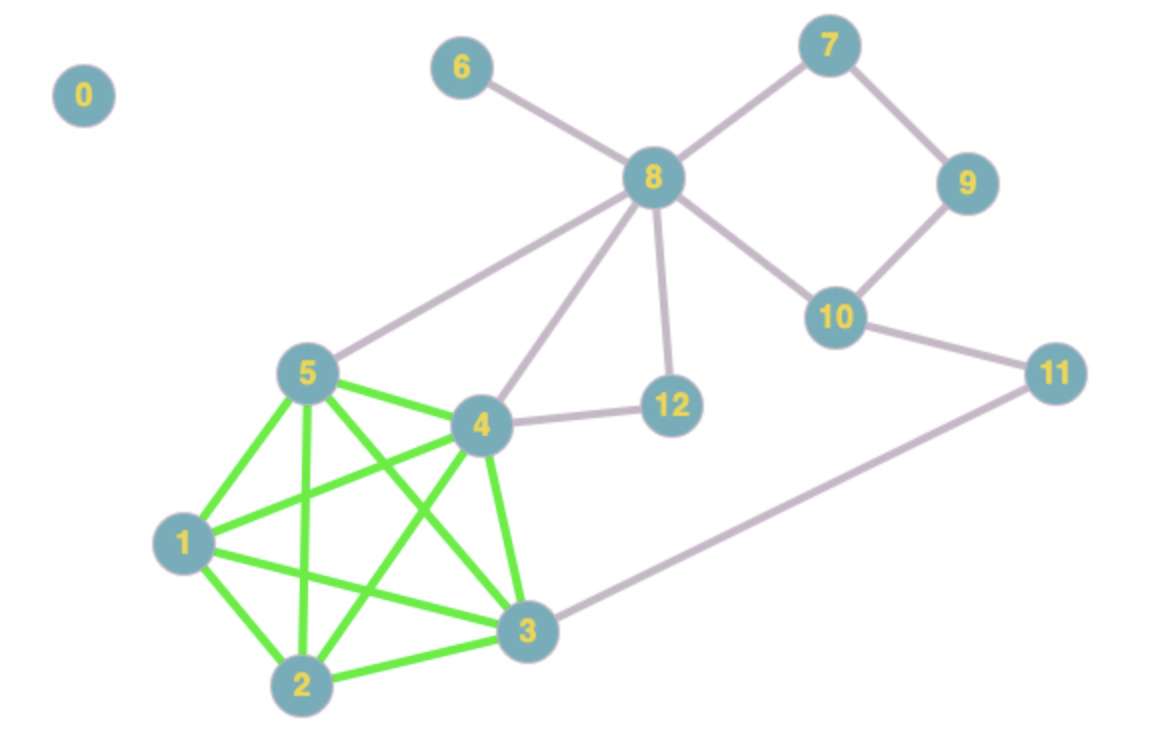
\includegraphics[width=0.7\textwidth]{img/connected_states.jpg}
    \caption{Example of a graph of States}
    \label{fig:connected_states}
    \end{figure}

    In the code, we have two parameters: first we have \texttt{Connections.CLUSTER\_SIZE} and then we have \texttt{Connections.PROB\_CONNECTION}. The former simply States how many States are present in the Cluster (for simpler analyzes later on, we have maximum one Cluster). We will make sure that all those States are correctly connected to one another. The second parameter simply State what is the probability of a State being connected to another when going through all States present in the World (\ref{section:world}). So, for instance, if we have a probability of 0.3, we will go through all the States of the World, and for each State, it has a probability of 0.3 to create a link with another State chosen at random. By doing this, some State will, possibly, be connected multiple times (i.e. two or more connections without being in a Cluster). This is a good thing as it will allow us to see the importance of the number of connections a State has (or whether it is in a Cluster).


\subsection{Market}\label{section:market}
The Market regroups all the products sold by the agents of one State, thus we have one Market for each State. Whenever a transaction takes place, the Market will compute the price of the exchange by including all the taxes (VAT, Tariff if the agents come from two different States which might not be connected). Whenever an agent wants to buy a Product, we will simply scan all the products available in the market and see which ones fit the demand by filtering on the price (buyer must have enough money) and the stocks of the product. To optimize this search, a HashMap has been created such that products are already sorted by their type and the search is, when profiled, \emph{much} faster, especially when we have tens of thousands of agents.

Whenever an agent wants to buy a product, we get a filtered list of all products the agent \emph{can} buy. There are multiple way of choosing a product from this list. Naturally, we could simply choose the cheapest one among those. However, other choosing methods have been developed to compare them. The other two methods are called \texttt{random} and \texttt{weightedRandom}. The former is rather obvious as we simply choose at random. This means that it is possible that the agent chooses the most expensive product (which is still affordable for the agent since the list has been previously filtered). The $3^{rd}$ method is a mix of the other two as we introduce some random but cheaper products have better chances at getting picked. The higher the price of the product, the less chances it will have at getting picked thanks because each product is associated with a probability which is inverse of its price.

\subsection{World Market}\label{section:WorldMarket}
The role of the World Market is simply to connected all the markets of all States because each Market only contains the products of the agents in that State, yet, agents can buy products from other States, which is why we need this link. Thus whenever an agent wants to make a purchase, we scan the markets of all States of the world and get a filtered list of products for each of them and simply combine them all into a single list of products to choose from. The World Market takes care of the transaction, the Gdp, the payments and other variables such as the black economy share depending which States the buyer and the seller belong to. It also allows us to get some interesting statistics such as the total number of purchases/transactions happening in the World.


\subsection{World}\label{section:world}
After describing all our models, we eventually finish with the one that will encompass them all: the World. The purpose of this model will be to initialize all products, agents and States as well as let them be inter-connected through the World Market.

The World will also handle the time step: a tick. Indeed, because computers are discrete machines, we have divide time into time steps (ticks). At each time step, our World will allow agents and States to perform actions such as producing, buying a product, collecting a tax or distributing allowances.

However, as previously expressed, not all agents will perform an action at every tick. Only a certain percentage of the agents will do something: either produce, or buy, or do nothing (in case it has no money to either produce or buy, therefore it waits for someone to buy one of its products or for the State to give him an allowance). However, the action of selling may happen at anytime. This means that an consumer will be able to buy a product from a seller without waiting for him to also perform an action (otherwise, the system would be blocked very often).
This percentage value will be rather small due to the fact that a tick is something that will happen very often.

Finally, because our World contains all of the models we have defined (i.e. the products, the agents, the States and the World Market), it will allow us to have an overview of all that is going on in our simulation. It will also be very useful in order to study the system and make some statistics. To compute these statistics, we will save all the key metrics of the World (e.g. number of transactions at a certain time/tick), the States (e.g. current Gini coefficient of all States), the Agents (e.g. initial and current money) and the Products (e.g. number of purchases and sales). 

These statistics are saved periodically after 100 ticks in case some error appears in the middle of the simulation. They are saved into \texttt{.csv} files which will then be analyzed later on so that we do not have to run the same simulation multiple times. 


\section{Running}
The project is freely available on Github at the following link: \url{https://github.com/RicGR98/MasterThesis}. All information to run the project are available in the \texttt{README.md} file in the root directory. A \texttt{run.sh} bash file has been created to run everything with a single simple command. This file works for local runs and also on the CECI cluster. Indeed, because these simulations are very computationally demanding, we have used the CECI (Consortium des Équipements de Calcul Intensif) cluster, ``funded by the Fonds de la Recherche Scientifique de Belgique (F.R.S.-FNRS) under Grant No. 2.5020.11 and by the Walloon Region''\footnote{\url{http://www.ceci-hpc.be/}}. For this, one has to copy the project files onto the cluster, then run \texttt{sbatch run.sh} and wait for the job to be launched by the cluster and let the simulation run for minutes, hours, or days (maximum 2) depending on the number of agents, states and ticks parameters. With the default parameters, it takes around 20 hours for all experiments to run parallelly on the CECI cluster. All commands to copy the files are available, as comments, at the end of the \texttt{run.sh} file.


\section{Class diagrams}

    To better understand how everything is linked and structured, we present now some class diagrams (from a large overview to a more detailed view). The class diagrams presented here are only for the Java code (thus for the simulation, not the experiments for instance)


    \begin{figure}[H]
        \centering
        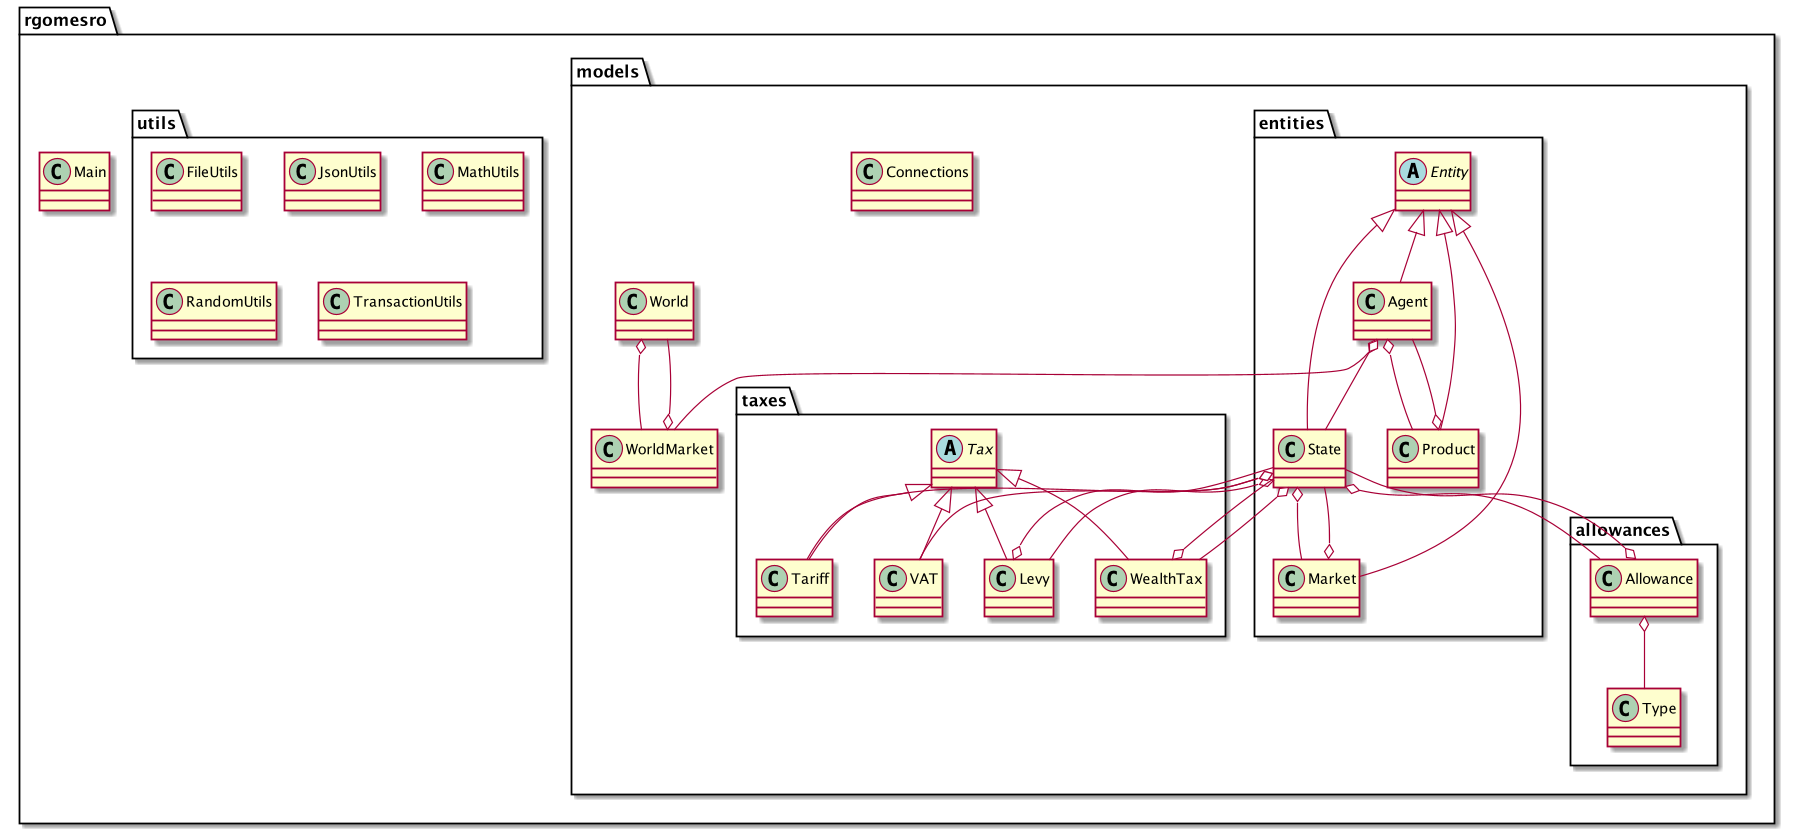
\includegraphics[width=1\textwidth]{img/generalCD.png}
        \caption{General class diagram}
        \label{fig:class_diagram_general}
    \end{figure}


    \begin{figure}[H]
        \centering
        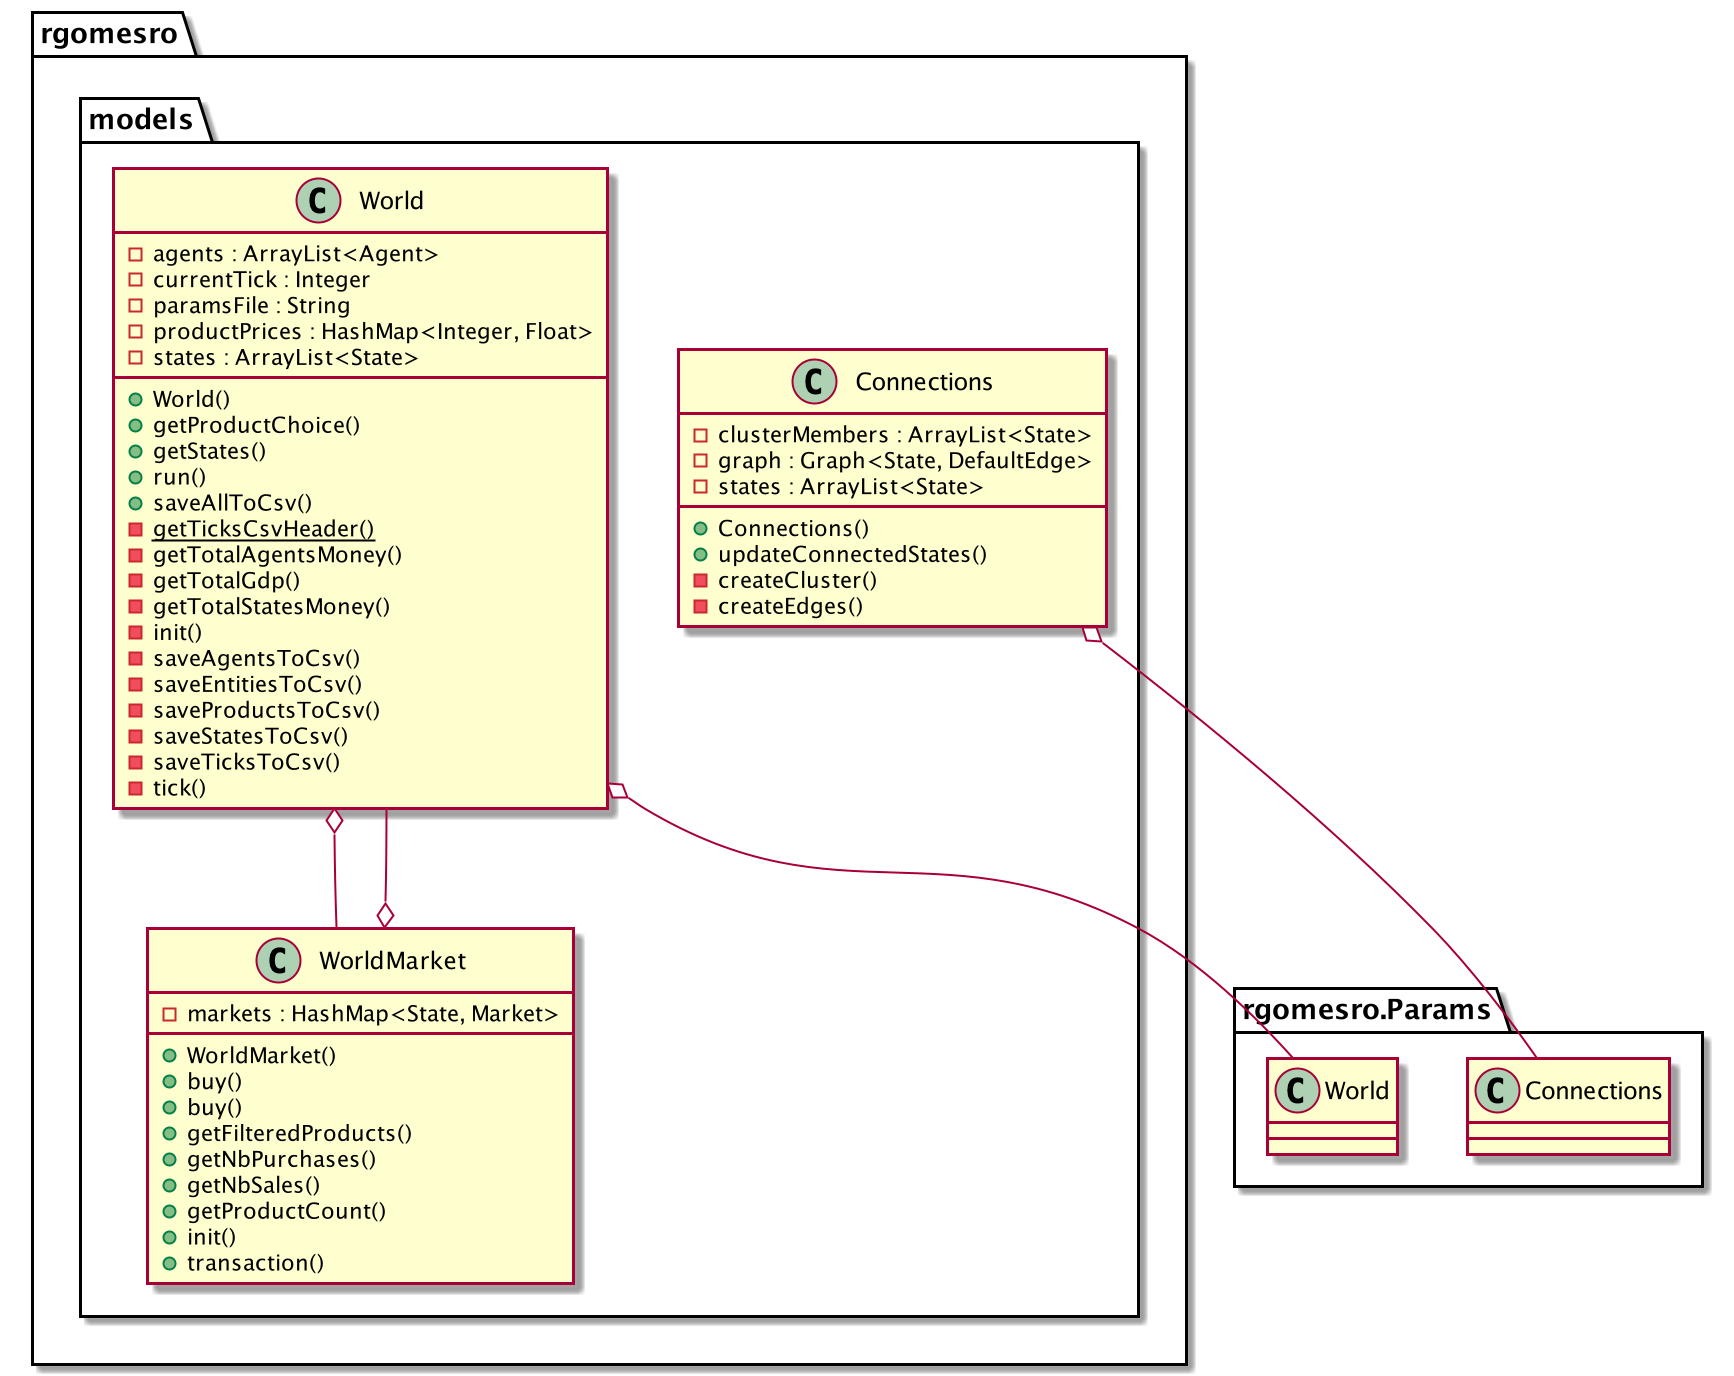
\includegraphics[width=1\textwidth]{img/modelsCD.png}
        \caption{Models class diagram (World, World Market and Connections)}
        \label{fig:class_diagram_models}
    \end{figure}


    \begin{figure}[H]
        \centering
        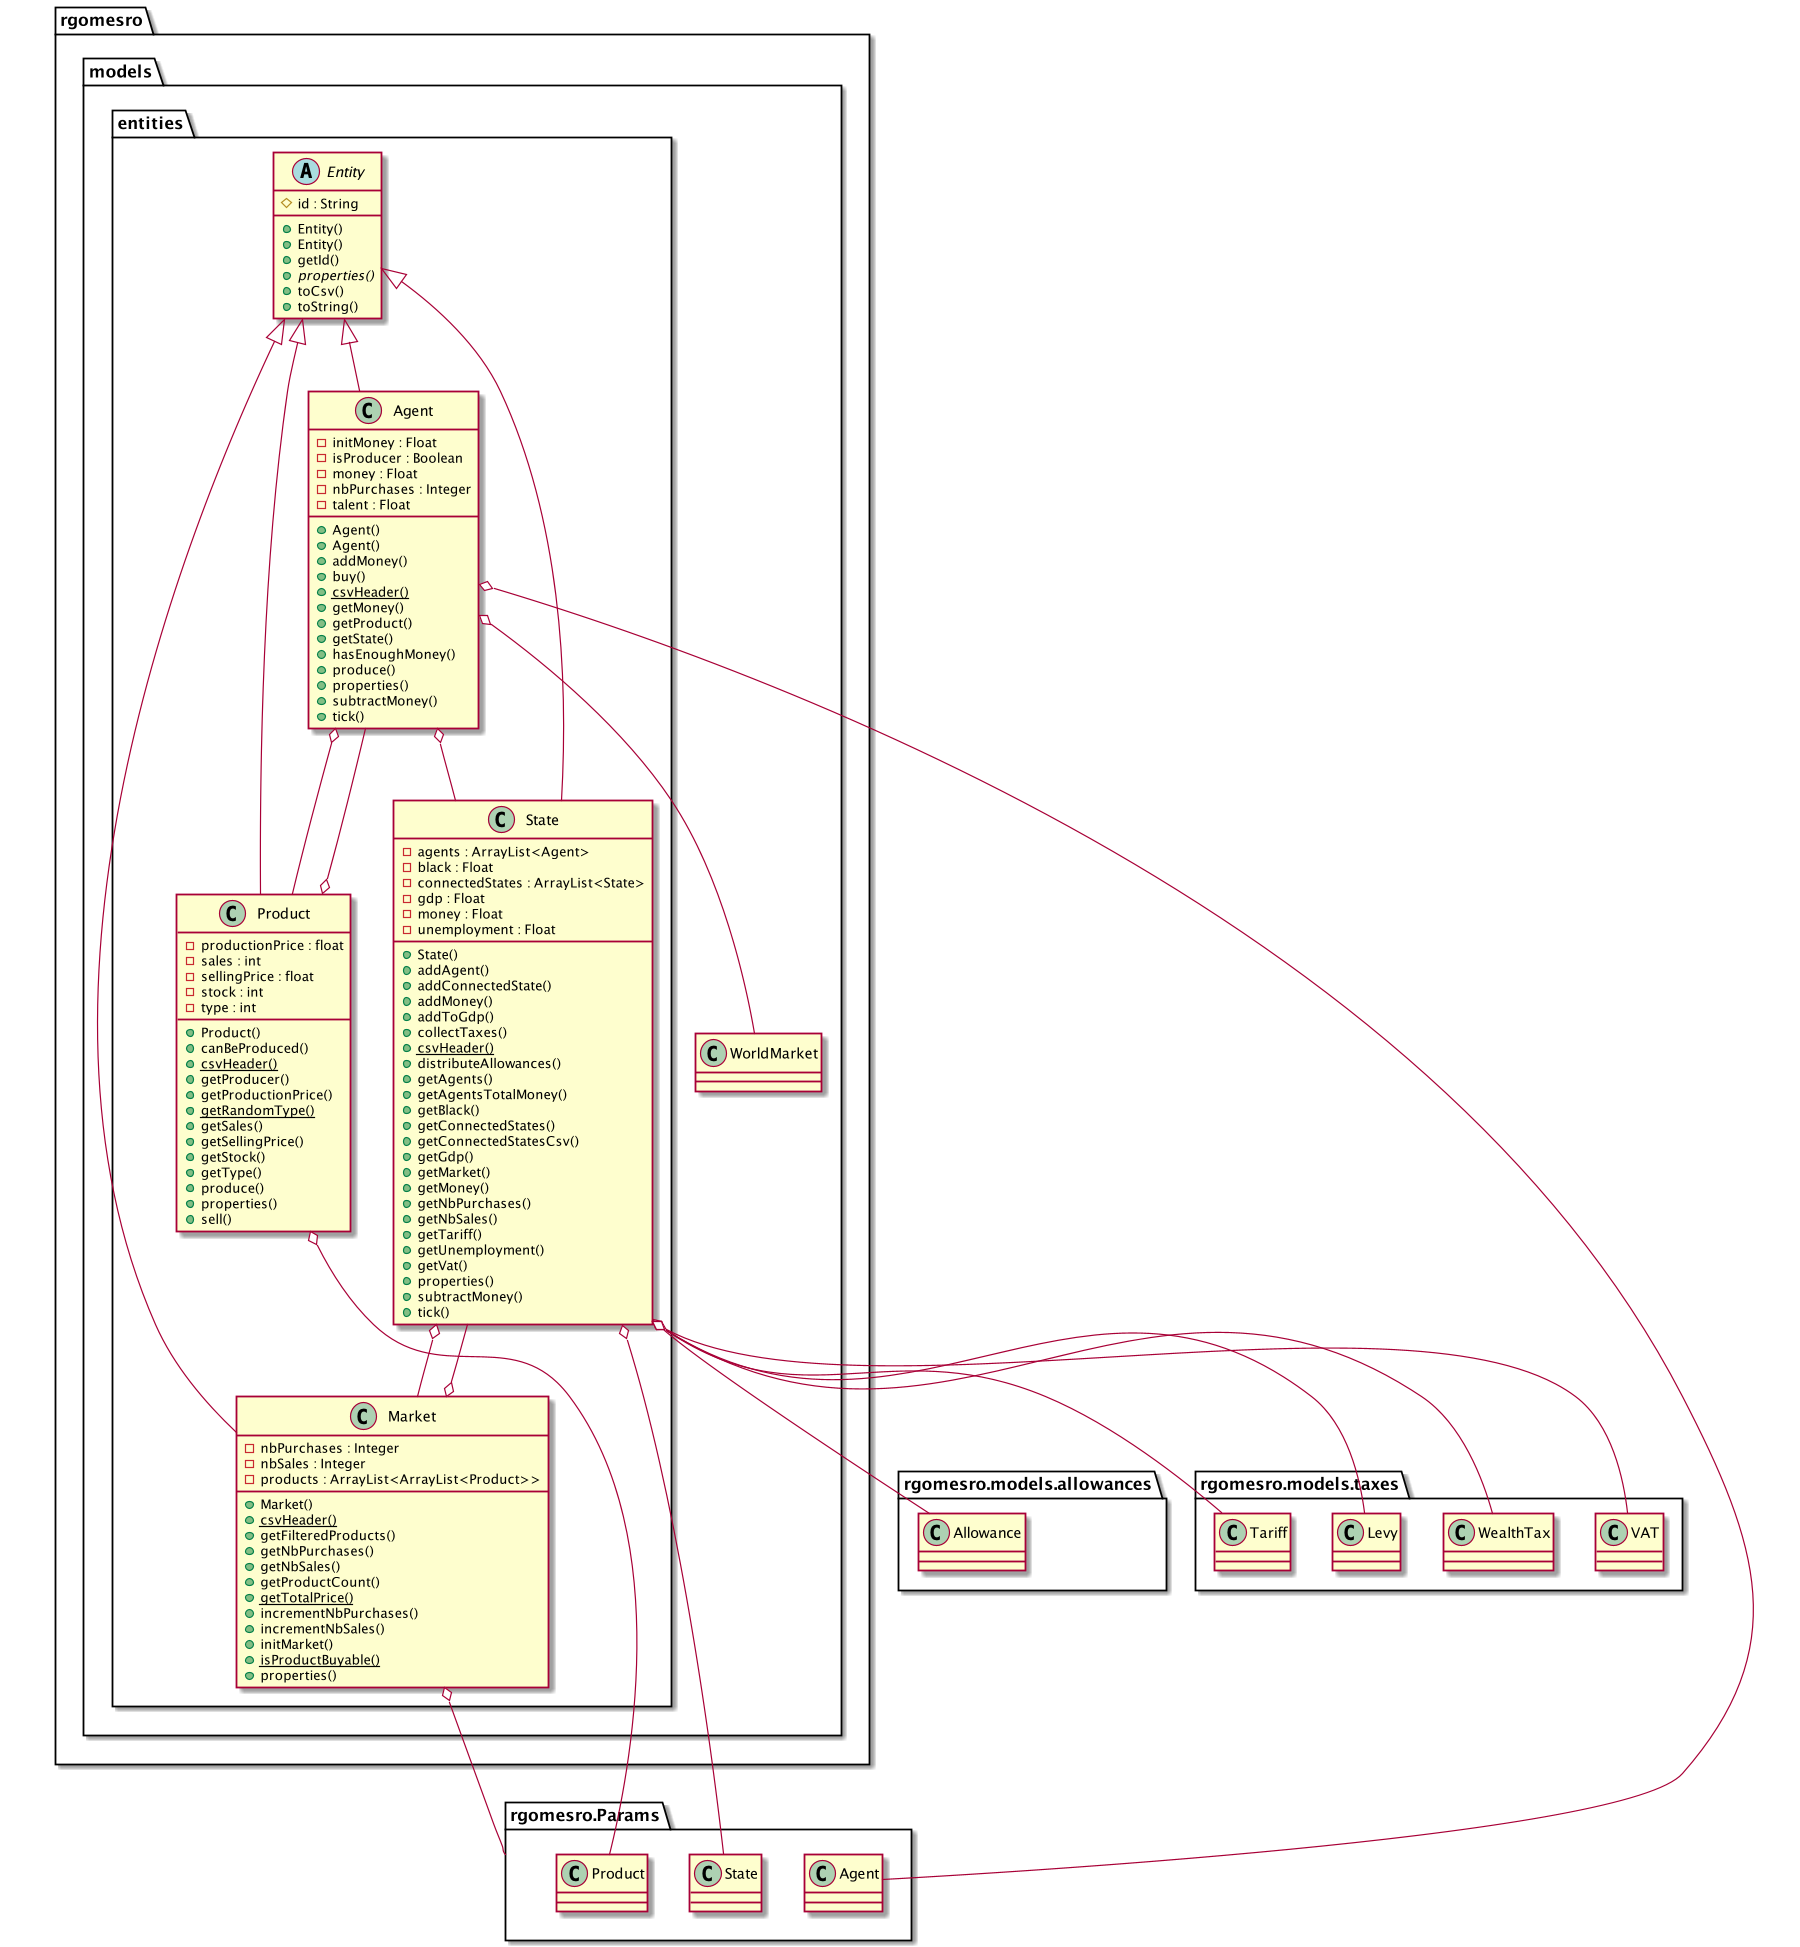
\includegraphics[width=1\textwidth]{img/entitiesCD.png}
        \caption{Entities class diagram (Agent, State, Product, Market)}
        \label{fig:class_diagram_entities}
    \end{figure}


    \begin{figure}[H]
        \centering
        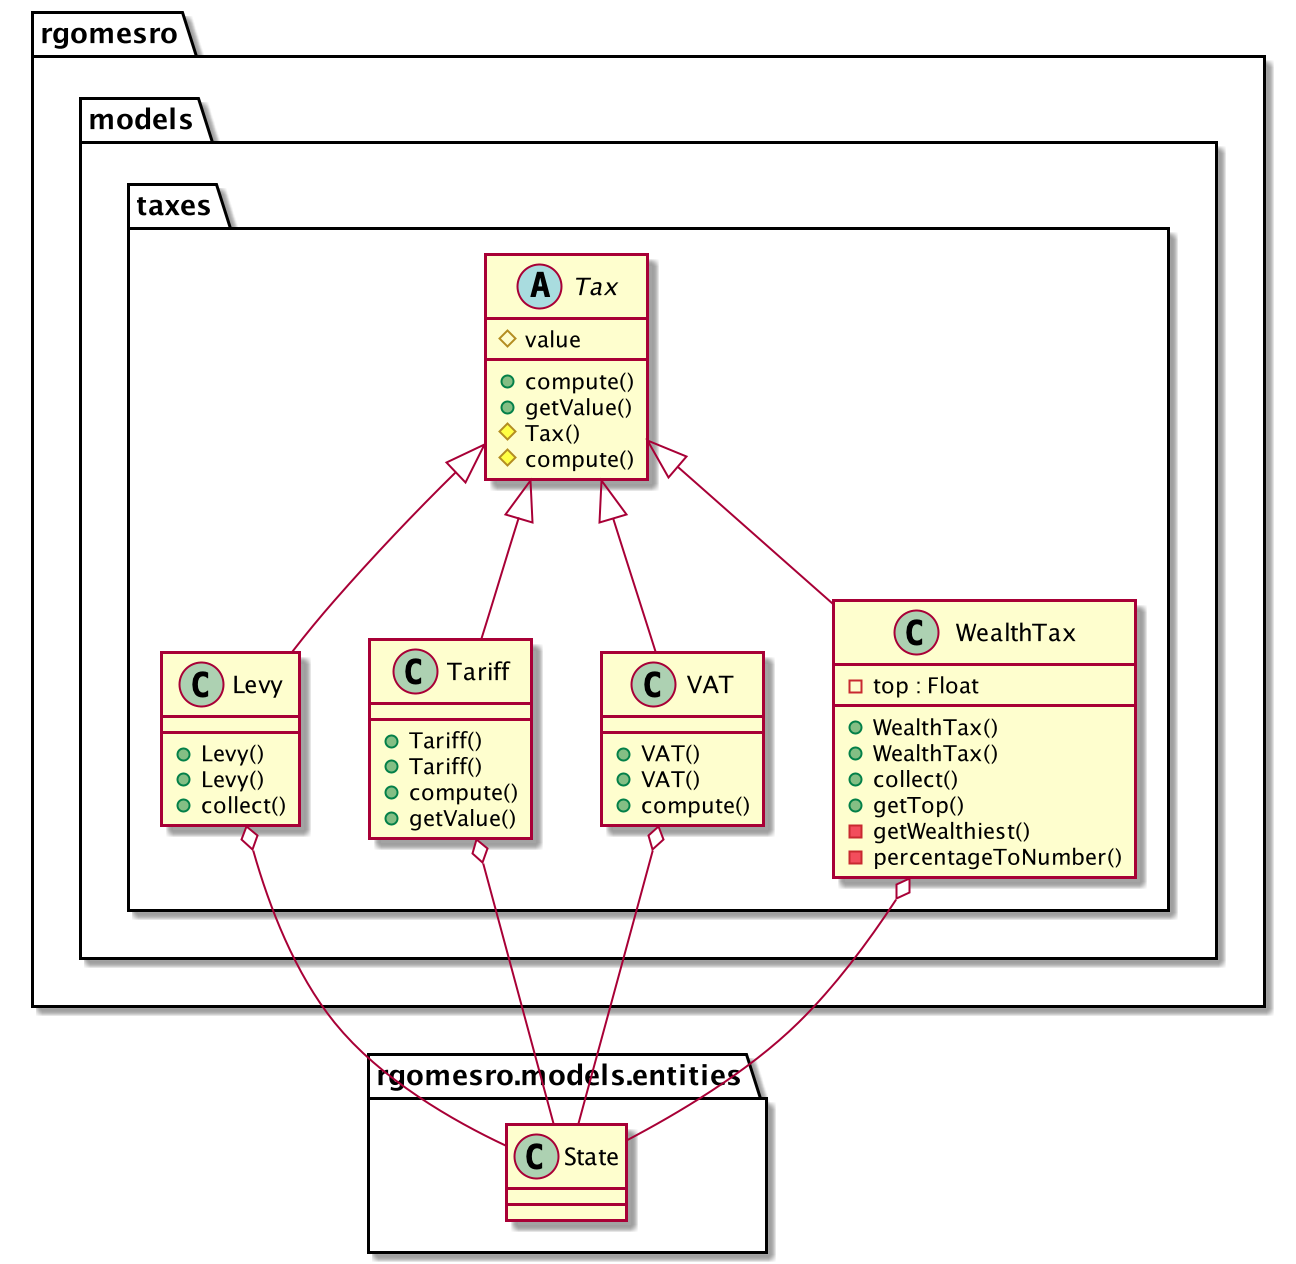
\includegraphics[width=0.7\textwidth]{img/taxesCD.png}
        \caption{Taxes class diagram (VAT, Levy, WealthTax, Tariff)}
        \label{fig:class_diagram_taxes}
    \end{figure}


    \begin{figure}[H]
        \centering
        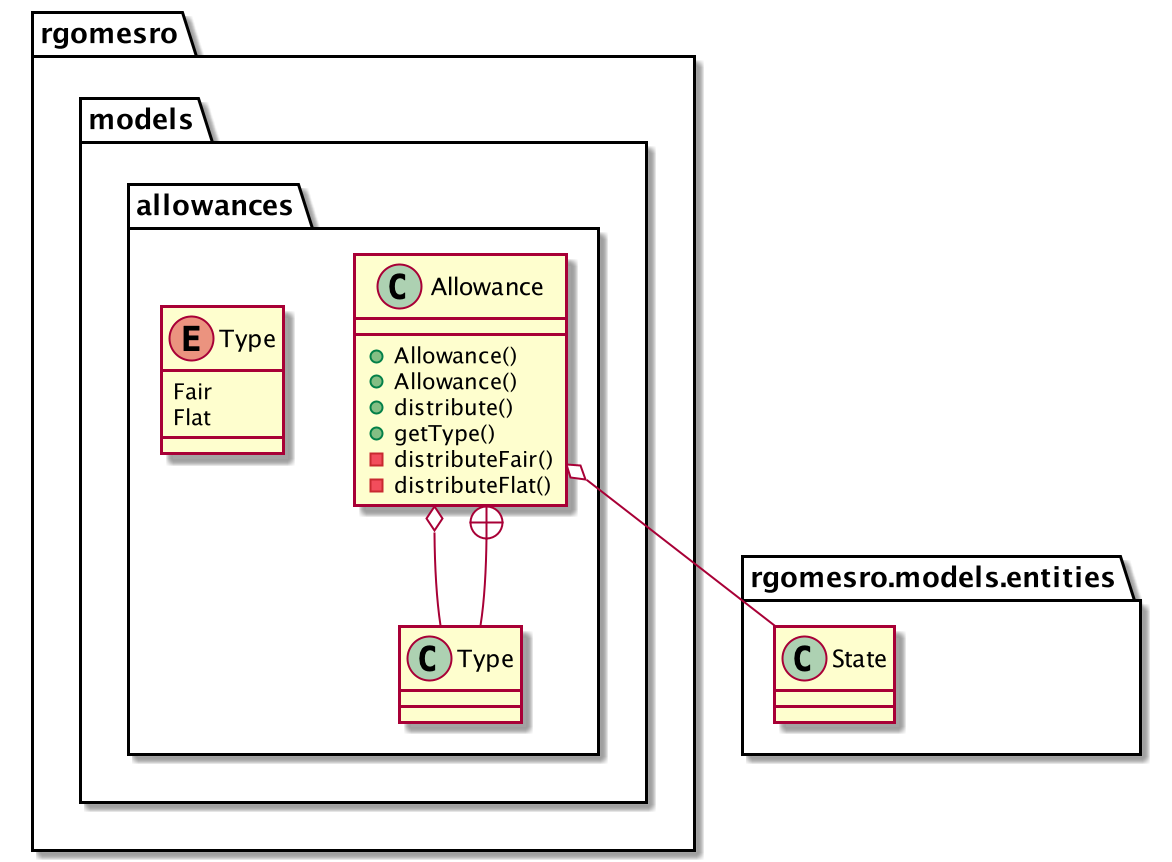
\includegraphics[width=0.7\textwidth]{img/allowancesCD.png}
        \caption{Allowances class diagram}
        \label{fig:class_diagram_allowances}
    \end{figure}
